% arara: xelatex
% arara: xelatex
% arara: xelatex


% options:
% thesis=B bachelor's thesis
% thesis=M master's thesis
% czech thesis in Czech language
% english thesis in English language
% hidelinks remove colour boxes around hyperlinks

\documentclass[thesis=M,english]{FITthesis}[2019/12/23]

%\usepackage[utf8]{inputenc} % LaTeX source encoded as UTF-8
% \usepackage[latin2]{inputenc} % LaTeX source encoded as ISO-8859-2
% \usepackage[cp1250]{inputenc} % LaTeX source encoded as Windows-1250

% \usepackage{subfig} %subfigures
% \usepackage{amsmath} %advanced maths
% \usepackage{amssymb} %additional math symbols

\usepackage{dirtree} %directory tree visualisation
% % list of acronyms
% \usepackage[acronym,nonumberlist,toc,numberedsection=autolabel]{glossaries}
% \iflanguage{czech}{\renewcommand*{\acronymname}{Seznam pou{\v z}it{\' y}ch zkratek}}{}
% \makeglossaries

% % % % % % % % % % % % % % % % % % % % % % % % % % % % % % 
% EDIT THIS
% % % % % % % % % % % % % % % % % % % % % % % % % % % % % % 
% \usepackage{pdfpages}
\usepackage{gensymb}
\usepackage{graphicx} %package to manage images
\graphicspath{ {./imgs/} }



\department{Department of Software Engineering}
\title{Log Server Analytics}
\authorGN{Daniil} %author's given name/names
\authorFN{Fedotov} %author's surname
\author{Daniil Fedotov} %author's name without academic degrees
\authorWithDegrees{Bc. Daniil Fedotov} %author's name with academic degrees
\supervisor{doc. Ing. Tomáš Vitvar, Ph.D.}
\acknowledgements{I would like to thank my supervisor doc. Ing. Tomáš Vitvar, Ph.D. for encouragement, 
	patient guidance and advices he has provided throughout the work.}
\abstractEN{Currently, information systems from the infrastructural point of view containing operating systems, web servers, application servers, load balancers, network communication elements produce a huge amount of operations data and write it to logs. Analysis of such logs can help to understand the current state of the system -- for instance, to determine the places, when errors occur. Such a knowledge helps to improve the performance of the system, make it more stable and accessible. Human is not able to read, analyze and process such a number of messages in a reasonable time, so it makes sence to perform a cluster analysis on server log files. Several groups (clusters) of similar log messages will be generated after clustering. This approach allows to significantly reduce the dimension of original log data, and allows to analyze not individual log entries, but groups, which siplifies searching and elimination of problems that have arisen during the server runtime. 
	
	This thesis proposes software for server log clustering based on natural language processing and machine-generated text processing techniques and machine learning algorithms, followed by the analysis of clustered log data. }

\abstractCS{V současné době informační systémy z pohledu infrasruktury zahrnují operační systémy, web servery, aplikační servery, prvky pro vyvažování zátěže a síťovou komunikaci, které produkují velké množství provozních dat a zapisují je do logů. Analýza takových logů pomáhá pochopit současný stav systému -- například, úrčit místa, kde vníkají chyby. Podobné ználostí pomáhájí vylepšit výkonnost stabilitu a dostupnost systému. Člověk nené shopen přečíst, analyzovat a zpracovavat velký počet zpáv v rozumnem čase, tedy má smysl provést sdružovací analýzu nad logovými soubry ze serverů. Výsledkem takové analýzy budou skupiny (shluky) podobných logových zpráv. Tento přístup dovolí výrazně snízit dimenze původních dat log a analyzovat skupiny místo jednotlivých zpráv logu, což zjednoduší vyhledávání a eliminaci problémů, které vníkaly během provozu serveru.
	
	Tato diplomová práce návrhuje software pro sdružovácí analýzu serverových logů, založený na metodách zpracování přírozeného jazyka, strojově-generovaných textech a algoritmech strojového učení s následující analýzou shluků logových dat.
  }
\placeForDeclarationOfAuthenticity{Prague}
\keywordsCS{Anal{\' y}za Log{\r u}, Zpracov{\' a}n{\' i} Log{\r u}, Logov{\' a} Data, Syst{\' e}my Zpracov{\' a}n{\' i} Log{\r u}, Anal{\' y}za Dat, Datov{\' a} V{\v e}da, Zpracov{\' a}n{\' i} P{\v r}{\' i}rozen{\' e}ho Jazyka, Strojov{\' e} U{\v c}en{\' i}.
	\\
	\\
	\\
	\\
}
\keywordsEN{Log Analytics, Log Processing, Log Data, Log Analytics Systems, Data Analytics, Data Science, Natural Language Processing, Machine Learning.}
\declarationOfAuthenticityOption{1} %select as appropriate, according to the desired license (integer 1-6)
% \website{http://site.example/thesis} %optional thesis URL


\begin{document}
% \newacronym{CVUT}{{\v C}VUT}{{\v C}esk{\' e} vysok{\' e} u{\v c}en{\' i} technick{\' e} v Praze}
% \newacronym{FIT}{FIT}{Fakulta informa{\v c}n{\' i}ch technologi{\' i}}


\setsecnumdepth{part}
\chapter{Introduction}

\section{Motivation}
In our days each organization uses complex software systems that makes business easier and much more productive. Such software systems typically consist of a number of services, databases and application servers, which are connected via the network and operate with a huge amount of data. Supporting these systems is a very complicated task. Each part of the system helps administrators to monitor the system state through generating logs, which describe every single activity performing on each particular part of the entire system.

Obviously, logs provide us with very useful information that needs to be stored and analyzed to keep the system in working state. The software size and complexity is continuously increasing that leads to rapid growth of log data. These massive amounts of logs need to be effectively processed and analyzed. One of the most important tasks needs to be done with logs is clustering -- partitioning log entries on several categories depending on the content of the message in the log entry.

Analysis of log data can be extremely helpful in situations, when some errors occur in the system. 

\section{Goal of the thesis}
The goal of the master thesis is to develop a system that will help to analyze and understand information provided by large logs generated by servers during runtime. To reach the goal the following tasks need to be done: 
%TODO the last goal may be modified
\begin{itemize}
	\item Define modern approaches in log server analytics, understand its concepts and principles,
	\item Explore the architecture of an environment with servers where log analitics will be performed,
	\item Design and implement a tool for log analytics that will be able to cluster log entries, 
	\item Analyze the acquired information to determine if there is a correlation between server load and generated logs.
	\item Evaluate the system and obtained results.
\end{itemize}
The tool should be provided as an installable package for the target systems.
\section{Thesis structure}
TO BE DONE



\setsecnumdepth{all}
\chapter{Basic concepts of Log Analysis}
\section {Log Analysis}
Log Analysis is a complex process of understanding of massive amounts of machine-generated texts, also known as log events or log entries, which provides useful information about how the components of the system works and what happens across the infrastructure. Typically, logs are streams of chronologically arranged messages which are generated by web servers, application servers, operation systems, elements of network communication etc. Log Analysis usually could be performed in the following several phases:
\begin{itemize}
	\item \textbf{Collecting} -- gathering all logs from all elements of the current infrastructure,
	\item \textbf{Centralization and indexing} -- this phase deals with transitioning of collected data to a centralized logging platform, where log entries will be normalized to a common format to ensure uniformity. Also, the log entries can be indexed to make searching more efficient. The described process simplifies the further querying and analysis,
	\item \textbf{Searching and analysis} -- searching for log entries which have a structure, defined by a pattern, or satisfied the queries,
	\item \textbf{Monitoring} -- monitoring helps to detect the anomalies occurrences in system runtime and determine how them impacted the performance. 
\end{itemize}
\section{Log Analysis core functions}
Log Analysis is a complex process that should follow the following functions:
\begin{itemize}
	\item \textbf{Pattern Detection and Recognition} -- filtering log entries based on a predefined patterns. Detecting patterns is an essential part of log analysis as it helps spot anomalies,
	\item \textbf{Log Normalization} -- conversion of individual log entry elements such as timestamps, IP addresses, machine IDs, messages, etc. to a common format,
	\item \textbf{Classification and Tagging} -- the process of tagging messages with keywords and categorizing them into separate classes. This allows to simplify and customize the further analysis and visualization,
	\item \textbf{Correlation Analysis} -- finding correlations among logs from different sources of the system infrastructure. Analysis of such correlations helps in finding similar behavior of the elements of the system. This information is very helpful when an incident occurs somewhere in the system. For instance, in the case of malicious activity, it allows to filter and correlate logs coming from the network devices, firewalls, servers, and other sources. Correlation analysis is usually associated with alerting systems – based on the pattern you identified, you can create alerts for when the log analyzer discovers similar activity in logs,
	\item \textbf{Artificial Ignorance} -- machine learning process that recognizes and discards log entries that are not useful. Typically, artificial ignorance is used to detect anomalies. That means to ignore routine messages generated from the normal operation of the system like regular system updates, thus labeling them as uninteresting. Artificial ignorance alerts about new and unusual events, even about common events that should have occurred but did not – for example, if a weekly updated has failed. Such an anomaly in system operation should be investigated \cite{sematext, xplg-site}.
\end{itemize}

\chapter{State-of-the-art}
\section{}

\chapter{Analysis and design}
Since technically logs are text streams or files it means that task of log processing is from text retrieval field. Text retrieval is a branch of information retrieval in which the information is stored primarily in the form of text \cite{text-retrieval-definition}. There are several steps specific to text retrieval tasks needs to be done proceeding to the analysis phase:
\begin{itemize}
	\item Text parsing,
	\item Normalization,
	\item Vectorization.
\end{itemize}
In the following sections every step is described in detail.

\section{Text parsing}
Log files gathered from different infrastructure components can significantly vary in formatting and semantics, but they still contain markers intended to separate individual elements within the data. Therefore, logs can be considered as semi-structured data \cite{semi-structured-data-graylog, semi-structured-data-definition}. 

In this work the logs from WebLogic Server are considered. 

The example of structure of the log message format is presented on figure \ref{fig:wls-log-entry-pattern}.

\begin{figure}\label{fig:wls-log-entry-pattern}
	\[<Timestamp> <Severity> <Subsystem> <Message ID> <Message Text>\]
\caption{WebLogic server log entry pattern}
\end{figure}

The description of each element of WebLogic Server log format is listed in table \ref{tab:log-format}

\begin{table}\centering
	\caption{WebLogic server log format description}\label{tab:log-format}
	\begin{tabular}{ |m{7em}|m{9cm}| }
		\hline
		\textbf{Attribute} & \textbf{Description}\\
		\hline
		Timestamp & The time and date when the message originated, in a format that is specific to the locale.\\
		\hline
		Severity & Indicates the degree of impact or seriousness of the event reported by the message.\\
		\hline
		Subsystem &	This attribute denotes the particular subsystem of WebLogic Server that was the source of the message. For example, EJB, RMI, JMS.\\
		\hline
		Server Name \newline
		Machine Name \newline
		Thread ID \newline
		Transaction ID & These four attributes identify the origins of the message. Transaction ID is present only for messages logged within the context of a transaction. Note: Server Name and Thread ID are not present in log messages generated by a Java client and logged to a client log.\\
		\hline
		Message ID & A unique six-digit identifier. Message IDs through 499999 are reserved for WebLogic Server system messages.\\
		\hline
		Message Text & For WebLogic Server messages, this contains the Short Description as defined in the system message catalog. For other messages, this is text defined by the developer of the program.\\
		\hline
	\end{tabular}
\end{table}
WebLogic Server subsystems or application code send log requests to Logger objects. These Logger objects allocate LogRecord objects which are passed to Handler objects for publication. Both loggers and handlers use severity levels and (optionally) filters to determine if they are interested in a particular LogRecord object. When it is necessary to publish a LogRecord object externally, a handler can (optionally) use a formatter to localize and format the log message before publishing it to an I/O stream. 

Figure \ref{fig:wls-logging} shows the WebLogic Server logging process. WebLogic Server subsystem or J2EE\footnote{J2EE -- Java Enterprise Edition} application invokes a method on one of logging implementations which distributes generated messages to to the server Logger object. The server Logger object publishes the generated messages to any message handler that has subscribed to the Logger.

\begin{figure}\centering
	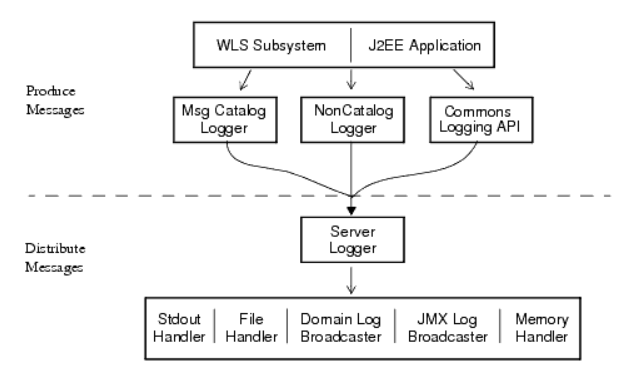
\includegraphics[scale=0.8]{wls-logging}
	\caption{WebLogic Server logging process}\label{fig:wls-logging}
\end{figure}

As it was described in table \ref{tab:log-format}, every log entry has a severity level attribute that indicates the potential impact of the event or condition that the message reports. All possible message severity levels are listed in table \ref{tab:wls-log-severity} arranged in ascending order.

\begin{table}\centering
	\caption{Message severity levels}\label{tab:wls-log-severity}
	\begin{tabular}{ |m{7em}|m{9cm}| }
		\hline
		\textbf{Severity} & \textbf{Meaning}\\
		\hline
		 TRACE & Used for messages from the Diagnostic Action Library. Upon enabling diagnostic instrumentation of server and application classes, TRACE messages follow the request path of a method. \\
		\hline
		 INFO & Used for reporting normal operations; a low-level informational message. \\
		\hline
		 NOTICE & An informational message with a higher level of importance. \\
		\hline
		 WARNING & A suspicious operation or configuration has occurred but it might not affect normal operation. \\
		\hline
		 ERROR & A user error has occurred. The system or application can handle the error with no interruption and limited degradation of service.\\
		\hline
		 CRITICAL & A system or service error has occurred. The system can recover but there might be a momentary loss or permanent degradation of service.\\
		\hline
		 ALERT & A particular service is in an unusable state while other parts of the system continue to function. Automatic recovery is not possible; the immediate attention of the administrator is needed to resolve the problem. \\
		\hline
		 EMERGENCY & The server is in an unusable state. This severity indicates a severe system failure or panic\cite{weblogic-log-structure}.\\
		\hline
	\end{tabular}
\end{table}

In this thesis the most interesting and important severity levels for further analysis and completion of defined tasks are warning and higher, but all severity levels are considered during the parsing phase. 

As it was described above log entries matches the pattern \ref{fig:wls-log-entry-pattern}, thus each log entry could be easily extracted from the log file and stored to proper object structure that could be conveniently processed in future.

% \section{Normalization}
% \section{Vectorization}
\chapter{Log Analytics techniques}
After we have defined the structure of the log files, it is time to move on to vectorization and the further analysis. Once logs are parsed and stored as structured objects in memory they needed to be transformed into numeric vector representation. This process is called feature extraction or vectorization. It is an essential first step in text analysis, and log analysis can be considered as a narrower field of text analysis.

Representing log messages numerically give us the ability to perform a meaningful analytics and compare vectors to each other. Each vector property is a feature representing attributes and properties of the log message. The obtained vectors can be considered as points in high-dimensional semantic space. Points in space can be close together or far apart, they may be tightly clustered or, on the contrary, evenly distributed. One of the most commonly used techniques for encoding of texts is the bag-of-words (BOW) model \cite{vectorization}. This model describes the occurrence of words within a document and involves the definitions of a vocabulary of known words and a measure of a presence of known words. The model concerns only with the presence of known words within the message, not the concrete place, where the word precisely occurs in the message \cite{bag-of-words}.

In this chapter a number of bag-of-words methods, which are used in this work, will be described.


\section{Natural Language Processing}
\textbf{Natural Language Processing (or NLP)} -- the branch of computer science and artificial intelligence that gives the computers the ability to understand texts and spoken words and derive meaning from human languages \cite{nlp-definition-tds, nlp-definition-ibm}. There are several tasks that are typical for NLP:
\begin{itemize}
	\item \textbf{Speech recognition} -- is a task of converting voice data to text data. Speech recognition is required for any application that follows voice commands or answers users' questions. The main difficulties in this task are fast talking, different accents and intonations, variety of slang,
	\item \textbf{Part of speech tagging}, or grammatical tagging, is the process of determining the part of speech of a particular word or piece of text based on its use and context,
	\item \textbf{Solving the problem of word sense disambiguation} -- determining the most appropriate meaning of the word with multiple meanings depending on the context \cite{nlp-definition-ibm},
	\item \textbf{Named entity recognition}, or NER, identifies and locates words or phrases as entities of real world such as person names, organizations, locations and so on \cite{ner-wiki},
	\item \textbf{Coreference resolution} is the task of finding expressions that refer to the same entity in a text. It is an important task needed to be solved before proceeding to the next analysis phase such as document summarization, question answering, or information extraction \cite{coreference-stanford},
	\item \textbf{Sentiment analysis} is a technique that is used to attempts to extract sentiment -- positive, negative, or neutral -- from given text \cite{sentiment-analysis-def},
	\item \textbf{Natural language generation} is the task of putting structured information into human language. This task can be considered as an opposite task to speech recognition \cite{nlp-definition-ibm}. 
\end{itemize}

There is a number of tools and approaches for NLP purposes. For instance, for Python programming language there is one of the most commonly used libraries in NLP field -- Natural Language Toolkit , or just NLTK. More information about the library can be found on \cite{nltk-homepage}. In this work NLTK library is used for NLP analysis method of log clustering.

\subsection{Linguistic approach} \label{sect:linguistic-approach}
To analyze the log data with BOW and NLP approaches, the raw text of log messages must be properly preprocessed. The common preprocessing process when solving NLP problems has the workflow as it is shown on Figure \ref{fig:nlp-workflow}% folowing workflow: 

% TODO draw a picture of the workflow and put it here

%\begin{itemize}
%	\item Tokenization,
%	\item Dimensionality reduction and normalization,
%	\item Encoding.
%\end{itemize}

\begin{figure}[h!]\centering
	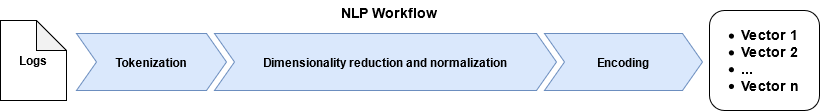
\includegraphics[scale=0.4]{nlp_workflow}
	\caption{NLP Workflow}\label{fig:nlp-workflow}
\end{figure}
Once the enumerated steps are done, every log entry from log file is repesented as a vector. In the following sections each part of this workflow will be described in details.
\subsection{Tokenization}
\textit{Tokenization} in common text processing meaning is a process of splitting the document into subsequences of characters that are grouped together as a useful semantic unit of processing. Such subsequences of characters are called tokens \cite{tokenization-def}. There are some options, how to split the text into tokens. The common practice in NLP area is word tokenization of text data. Thus, applying this approach to log entries there will be a set of vectors consisting of individual words obtained from log entries' message part. 

\subsection{Dimensionality reduction and normalization}
Due to the logs' nature, along with human-readable text in their messages, they contain a lot of technical details and redundant information from a semantic and linguistic points of view. So, for example, typical error message written in the log contains a stack trace that helps technical experts to locate the error and determine its root cause. Stack traces always have the information about numbers of rows in source code, where the exception were thrown, often there are paths to files in error's description, special symbols and so on. But since we are speaking of semantics, such information is not necessary and may be removed from the message since it is more important to understand the meaning of the error. Removing non-meaningful data and getting the tokens to a consistent state is called \textit{normalization}.  

The vast majority of software produces the logs in English language. From the perspective of this language there are lots of commonly used words (such as "is" "the", "a", "an", "in" etc.) that have very little meaning and do not add much information to the text. By removing these words, qualitatively there is no loss of information. On the contrary, there is a focus on more valuable and meaningful information.

Typically, all messages in log entries contain some punctuation. Coming back to stack trace example, it could be seen that there are lots of dots, colons, semicolons etc. in there. Punctuation is an important part of any language , however, it is not interesting for our analysis.

Next step in the preprocessing phase is getting the obtained on previous phase words into consistent normalized state. To achieve this state there are commonly used techniques -- stemming and lemmatization.

\textit{Stemming} is a process of transforming related or similar variants of a word to its base form to which suffix can be attached, as they share the same meaning \cite{stemming-def}. Thus, stemming transforms words to its parts that never changes. For example, for word \textit{"waiting"} the stem will be \textit{"wait"}, for word \textit{"connection"} the stemmed version is \textit{"connect"}. In common case stemming a word may result in words that are not actual words, for example, for word \textit{"computer"} the stem is \textit{"comput"}, since there are forms \textit{"computing"}, \textit{"computed"}, \textit{"computation"}.

One of the most famous and commonly used stemming algorithms is \textit{Snowball Stemming Algorithm} derived from older Porter Stemming Algorithm proposed by Martin Porter \cite{porter-stemming-alg}. The original Porter algorithm suffered from some issues that were fixed in Snowball. For example, when applying Porter Stemming Algorithm on words \textit{"fairly"} and \textit{"sportingly"} the result will be \textit{"fairli"} and \textit{"sportingli"} respectively, but the results for Snowball algorithm for these words will be \textit{"fair"} and \textit{"sport"} \cite{snowball-porter-difference}. 

Another dimensionality reduction NLP technique is \textit{lemmatization}.  
Unlike stemming lemmatization usually refers to return the base or dictionary form of a word with the use of a vocabulary and morphological analysis. Such a base form is called lemma. There is an example given to clearly see the difference between stemming and lemmatization. For the word \textit{"saw"} stemming algorithm will return just \textit{"s"}, but the result of the lemmatization algorithm will be \textit{"see"} \cite{stemming-and-lemmatization}.

So, when the both dimensionality reduction techniques have been discussed, there is a question when to use each of them, and which one is more relevant for the log analytics task. When the speed is prefered over the linguistics then stemming should be used since lemmatiztion algorithms scan a corpus of words which is a time consuming task. But when the problem is more linguistic and when it is necessary to preserve language norms, preference should be given to lemmatization \cite{stemming-or-lemmatization}. In the problem of log analysis stemming approach is more preferable then lemmatization since log messages are mostly written for technical experts who can read and understand it that is such messages may not preserve the language rules and norms. Moreover, the speed of processing the log messages is very important as well, because in the enterpise infrastructure all elements produce massive amounts of logs that must be processed in a reasonable time. 

In this master thesis stemming is used as a dimesionality reduction technique.

\subsection{Encoding}
After dimensionality reduction phase it's time to proceed to conversion arrays of tokens into numerical vectors. \textit{Vector Space Model} is an algebraic model for encoding text documents as vectors \cite{vsm-wiki-def}. There is a number of vectorization techniques and the choice of a specific one is largely driven by the problem domain. In this paragraph three commonly used approaches to text vectorization will be presented.

\subsubsection{Term Frequency Vectorization}\label{sect:tf-vectorization}
The first vectorization approach is based on measurement of terms (tokens) frequencies within a document (or a message in case of log entries). According to this vectorization the resulting vector for every log message will be filled with the frequency of each word appears in the log message. The vectors can be straightly counted or normalized with weighting each word by the total number of words in the message. The example of term frequency vectorization is depicted on \ref{fig:term-frequency}.

%TODO draw a picture of such an approach like it is done by O'Reilly below.
\begin{figure}[h!]\centering
	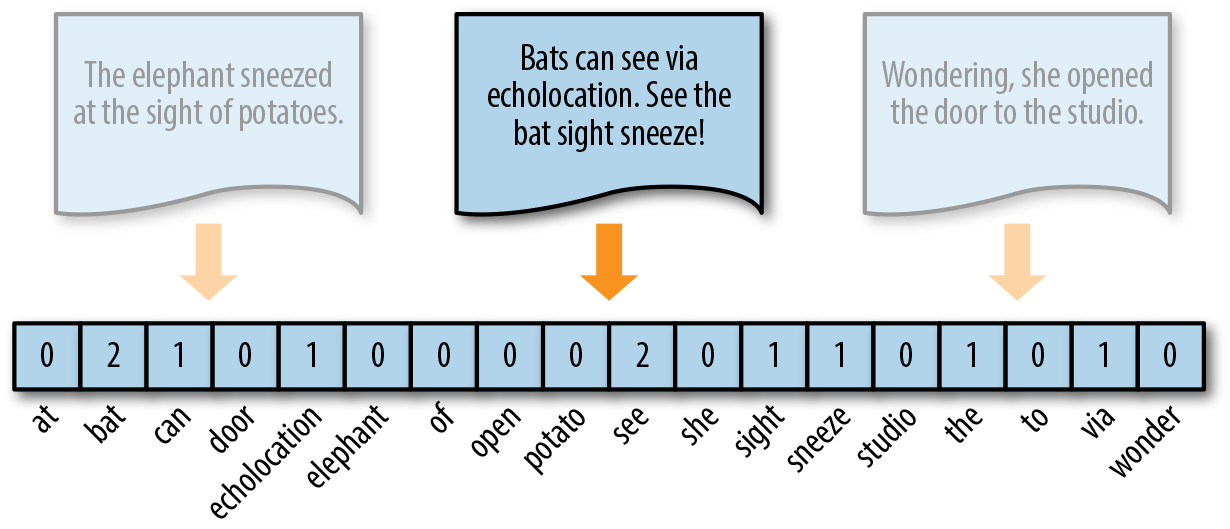
\includegraphics[scale=0.8]{term-frequency}
	\caption{Term Frequency Vectorization}\label{fig:term-frequency}
\end{figure}

Term Frequency approach is widely used, but it has a drawback. Tokens that occur very frequently could be considered as more "significant" then other ones, which occur less often\cite{vectorization}. That does not always correspond to reality. 

\subsubsection{One-Hot Vectorization}
One-Hot vectorization is a vector of boolean values. Each such value only indicates the presence of the token within a message. \textit{True (1)} value stands for presence and \textit{Flase (0)} stands for absence of the token as it is represented on \ref{fig:one-hot}.
%TODO draw a picture of such an approach like it is done by O'Reilly below.
\begin{figure}[h!]\centering
	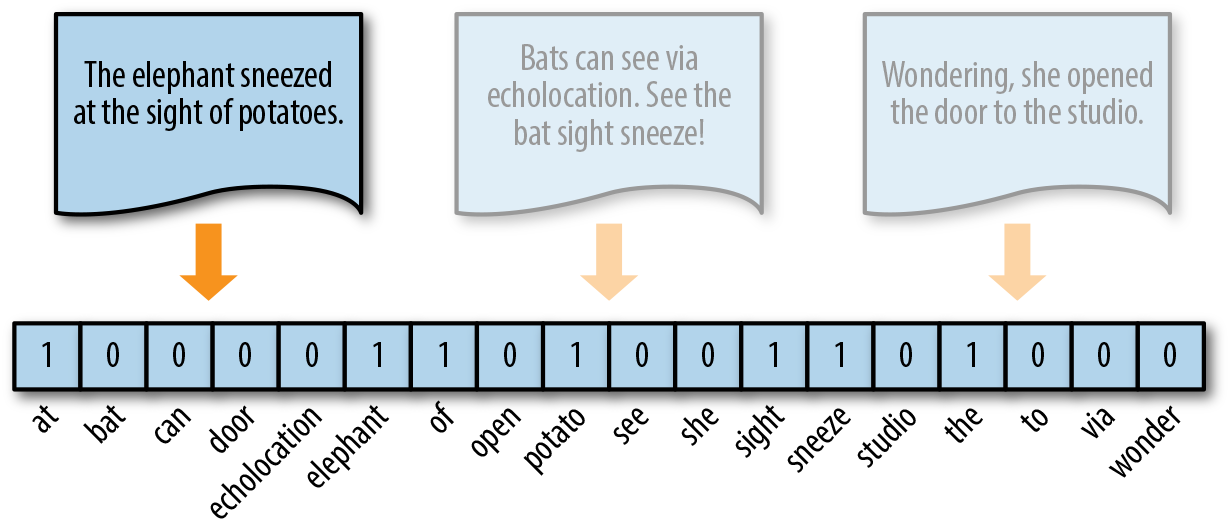
\includegraphics[scale=0.8]{one-hot}
	\caption{One-Hot Vectorization}\label{fig:one-hot}
\end{figure}
Although, it seems to be a good model since it is very simple and transparent, but it is not convenient, because it does not scale well when a large corpus is given, and it disregards the semantics, thus it is not commonly used in NLP tasks. And it is not suitable for log analytics purposes, because of massive amounts of log data. Thus, vector for each log entry would be extremely highly dimensional and sparse, resulting in increased time and computational complexities.


\subsubsection{Term Frequency - Inverse Document Frequency}
The BOW representations that were considered so far only describe a document in a standalone fashion, not taking into account the context of the corpus. A better approach is to consider the relative frequency or rareness of tokens in the log message against their frequency in other log messages. The main idea is that the meaning is most likely encoded in the more rare terms from a log message. 
For example, in a corpus of error log messages, tokens such as "input", "output", and "stream" appear more frequently in log entries describing \textit{IOException\footnote{IOException -- Signals that an I/O exception of some sort has occurred. This class is the general class of exceptions produced by failed or interrupted I/O operations \cite{oracle-ioexception}.}}, while other tokens that appear frequently throughout the corpus, like "exception",  "weblogic", and "java”", are less important.

%TODO draw a picture of such an approach like it is done by O'Reilly below.
\begin{figure}[h!]\centering
	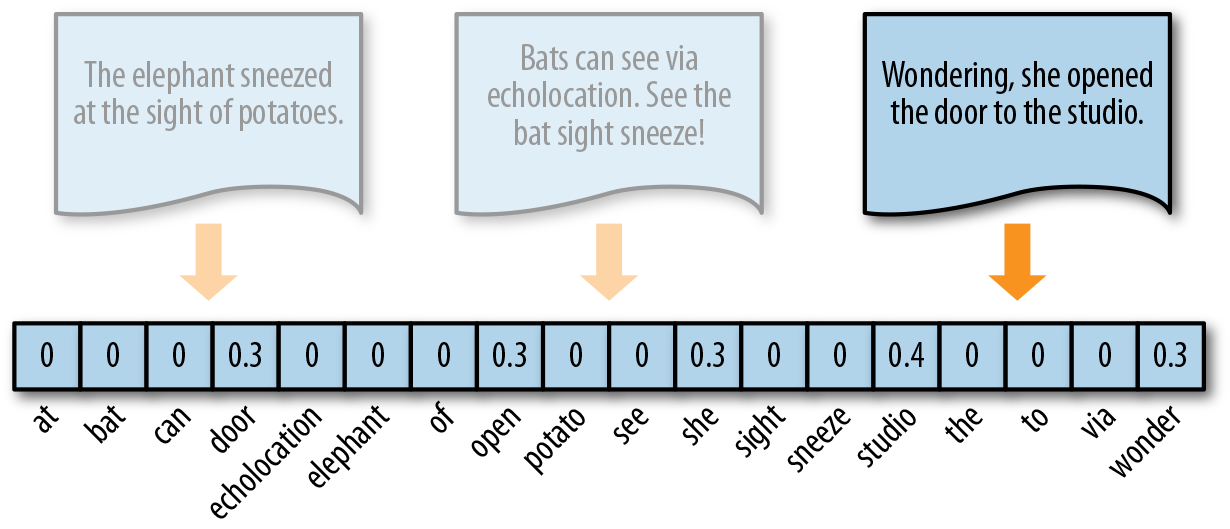
\includegraphics[scale=0.8]{tf-idf}
	\caption{Term Frequency - Inversed Document Frequency}\label{fig:tf-idf}
\end{figure}

\textit{\textbf{Term Frequency – Inverse Document Frequency (TF-IDF)}} vectorization technique normalizes the frequency of terms (tokens) in a log entry message with respect to the rest of the corpus. This approach emphasizes terms that are very relevant to a specific instance, as shown in figure \ref{fig:tf-idf}, where the term has a higher relevance to this message since it only appears there\cite{vectorization}. 

\textit{\textbf{Term Frequency (TF)}} -- the number of times a term appears in a message, divided by the total number of terms in that message. The division is necessary since the larger messages likely contain more occurrences of the term, so it must be normalized as shown Formula \ref{eq:tf}.
%TODO check how the formulas are presented in other works
\begin{equation}\label{eq:tf}
	TF(t, m) = \frac{n_t}{N},
\end{equation}
where
\begin{itemize}
	\item \(t\) -- the considering term,
	\item \(m\) -- the message containing the considering term,
	\item \(n_t\) -- the number of times term \(t\) appeared within the message \(m\),
	\item \(N\) -- the total number of terms in the message \(m\).
\end{itemize}

\textit{\textbf{Inverse Document Frequency (IDF)}} -- measures the importance of the token. It is computed as the logarithm of the number of the messages in the corpus divided by the number of messages where the specific token appears (Formula \ref{eq:idf}).
%TODO check how the formulas are presented in other works

\begin{equation}\label{eq:idf}
	IDF(t, M) = \frac{|M|}{|\{m_i \in M | t \in m_i\}|},
\end{equation}

where 
\begin{itemize}
	\item \(t\) -- the considering term,
	\item \(M\) -- the corpus,
	\item \(|M|\) -- the number of messages in the corpus,
	\item \(|\{m_i \in M | t \in m_i\}|\) -- the number of messages from the corpus \(M\) where the term \(t\)  appears.
\end{itemize}

Thus, the resulting \textit{TF-IDF} measure for the term \textit{t} within the message \textit{m} is a product of \textit{TF(t, m)} and \textit{IDF(t, M)} as shown Formula \ref{eq:tf-idf}\cite{tf-idf-def}.
\begin{equation}\label{eq:tf-idf}
	\textit{TF-IDF}(t, m, M) = TF(t, m) \times IDF(t, M)
\end{equation}

Due to its ability to focus on important terms relevant to the considering message and pay less attention to more frequent terms of the whole corpus, \textit{TF-IDF} is a good choice for the log messages vectorization.

\subsection{Summary}
In this section, the log entries processing from the principles of natural language processing point of view was described. The transformation of the log messages into token arrays is considered, methods of dimensionality reduction, such as stemming and lemmatization, are presented, and the bag-of-word text vectorization techniques (Term Frequency Vectorization, One-Hot Vectorization and Term Frequency - Inverse Document Frequency) are discussed.

All methods have their advantages and disadvantages. The best linguistic approach workflow for log analysis is the following:
\begin{itemize}
	\item Word tokenization,
	\item Removing numbers and stop words,
	\item Stemming as a dimensionality reduction technique,
	\item \textit{TF-IDF} as a vector space model.
\end{itemize}


\section{N-grams approach}\label{sect:n-grams-approach}
As it was already mentioned logs are machine-generated texts which are not readable and understandable by a regular user of the system. The previous log analytics approach was based on the assumption that similar log entries have similar semantic structure and preserve the meaning. In this section another approach will be considered which is focused on logs' machine-generated nature. Instead of word tokenization followed by the dimensionality reduction techniques such as stemming and lemmatization, in this section an approach based on \textit{N-grams} will be considered.

\subsection{N-grams tokenization}
In computational linguistics area, an \textit{N-gram} is an overlapping sequence of n tokens from a given sample of text or speech \cite{n-grams-wiki}. It does not matter what the tokens are, it can be phonemes, syllables, letters, words or base pairs according to the application, where the N-grams are used. 

Unlike the previous linguistic method, where the log messages were tokenized into individual words, this method tokenization will rely on symbols.

Depending on the value of the \textit{N} parameter uni-grams, bi-grams, tri-gram and so on are distinguished. There are two main benefits of using n-grams -- implementation simplicity and scalability. With the larger \textit{N} such a model can store more context information, that in certain cases may improve the results. The examples of uni-grams, bi-grams, and tri-grams tokenizations are presented on Figure \ref{fig:uni-grams}, Figure \ref{fig:bi-grams}, and Figure \ref{fig:tri-grams} respectively.

\begin{figure}[h!]\centering
	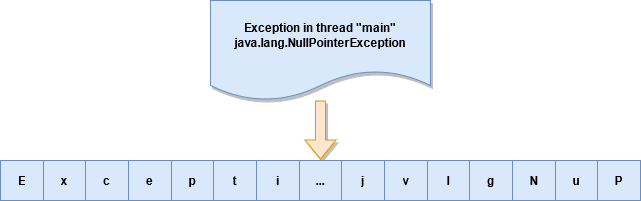
\includegraphics[scale=0.48]{uni_grams}
	\caption{Tokenization using uni-grams}\label{fig:uni-grams}
\end{figure}

\begin{figure}[h!]\centering
	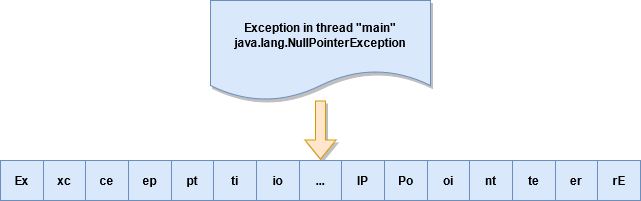
\includegraphics[scale=0.48]{bi_grams}
	\caption{Tokenization using bi-grams}\label{fig:bi-grams}
\end{figure}

\begin{figure}[h!]\centering
	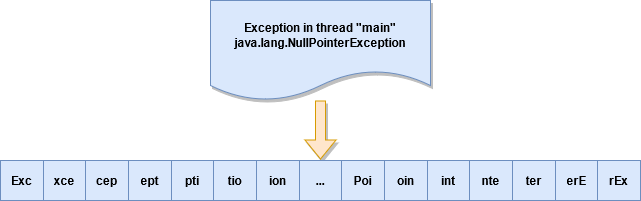
\includegraphics[scale=0.48]{tri_grams}
	\caption{Tokenization using tri-grams}\label{fig:tri-grams}
\end{figure}

\subsection{Dimensionality reduction and normalization}
As for the linguistic method the N-grams require dimensionality reduction as well. But since this approach is a more "machine" than the previous one, there is no need for stop words removing, CamelCase notation parsing, stemming, and lemmatization. The only normalization steps that can be applied are numbers and punctuation removing. 

These steps can help to significantly reduce the dimensionality of resulting N-grams vectors.

\subsection{Encoding}


Vectorization of log messgages can be done similarly to \textit{Term Frequency Vectorization} that was described in \ref{sect:tf-vectorization}, but with N-grams as tokens. Hence, for each N-gram the number of its appearances is computed. On the figure \ref{fig:bi-grams-vec} the bi-grams vectorization is depicted. The resulting values can be normalized with weighting each N-gram by the total number of N-grams in the message.

\begin{figure}[h!]\centering
	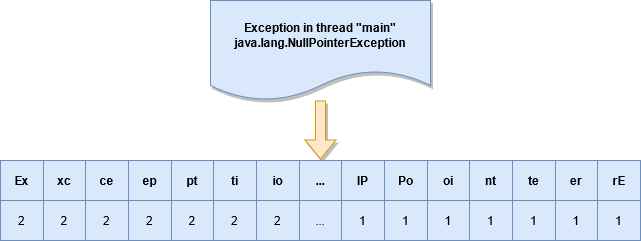
\includegraphics[scale=0.48]{bi_grams_vec}
	\caption{Vectorization using bi-grams}\label{fig:bi-grams-vec}
\end{figure}


\subsection{Summary}
In this thesis bi-grams of symbols are used as tokens. Such a choice is justified by the fact that uni-grams of symbols do not describe the log messages enough precisely, it is just a count of individual symbols, that reliable for further message comparison. Tri-grams, four-grams and so on significantly increase sparsity of resulting vectors since with increasing N-gram the number of repetitions of such an N-gram within the log message is reduced. Thus, bi-grams ensures the best coverage of the log messages.

\section{Clustering}
In previous sections log analysis two approaches that are used in this thesis were discussed in detail. Now, it is time to proceed to clustering.

One of the tasks in this thesis is clustering analysis. Cluster is a structure containing similar log entries. In order to group log entries into the same cluster, it is necessary to compare vectors with each other to determine how similar they are.

In data analytics area there are two main approaches to vectors comparison, distance and similarity. Distance measures how the two vectors are close to each other in the vector space, when similarity measures how two vectors are similar.

One of the most commonly used similarity measures in clustering analysis is cosine similarity.

Let two vectors \textbf{A} and \textbf{B} be given. The angle between them equals to \(\theta\) (Figure \ref{fig:cos_sim}). 

\begin{figure}[h!]\centering
	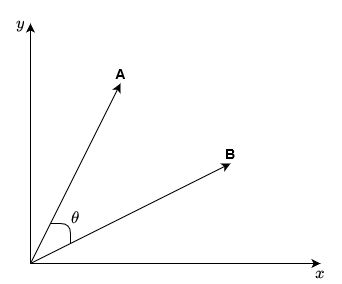
\includegraphics[scale=0.6]{cos_sim}
	\caption{Angle between two vectors \textbf{A} and \textbf{B}}\label{fig:cos_sim}
\end{figure}

Mathematically, it measures the cosine of the angle between two vectors projected in a multi-dimensional space (Formula \ref{eq:cosine-similarity}).

\begin{equation}\label{eq:cosine-similarity}
	sim(\textbf{A}, \textbf{B}) = cos(\theta) = \frac{\textbf{A} \cdot \textbf{B}}{||\textbf{A}|| \cdot ||\textbf{B}||},
\end{equation}
where 
\begin{itemize}
	\item \(\textbf{A}\), \(\textbf{B}\) -- the considering vectors,
	\item \(||\textbf{A}||\), \(||\textbf{B}||\) -- lengths of the \(A\) and \(B\) vectors respectively.
\end{itemize}

If two vectors are identical, then the angle between two vectors is \(0\), hence, \(cos(0\degree) = 1\), and vice versa when two vectors are completely different, then \(cos(90\degree) = 0\)

The cosine similarity is advantageous because even if the two similar documents are far apart by the  distance measure because of the size they could still have a smaller angle between them. The smaller the angle between the vectors, the higher their similarity \cite{cos-similarity}.

Cosine similarity is used in this thesis as a similarity measure for making clusters of similar log entries.

% A plenty of distance metrics exist. Some of them are for more general purposes, some of them are for more specific tasks.  <--- Move it to Neural Network chapter and describe there Minkowski distance, Manhattan distance and Euclidean distance.

\chapter{Log Analytics and Machine Learning}
In our days Machine learning is a rapidly growing area. Many algorithms have emerged based on the principles of machine learning, which are actively used in the development of new services, such as email filtering, digital assistants, product recommendation, practical speech recognition, effective web search, fraud detection, and so on \cite{ml-use-cases}.

One of the most interesting and perspective branches of machine learning is \textit{artificial neural networks}.

Artificial neural networks (ANN) are a subset of machine learning algorithms, which conceptually work similarly to human's brain. ANN consists of a set of so called \textit{"neurons"}. A neuron actually is a mathematical function that collects and processes the information according to a specific architecture. Neurons are interconnected, and their interconnection may vary depending on type of ANN and the solving problem\cite{nn-basics}.

The problem of data cluster analysis can be solved with machine learning techniques as well. In this chapter a machine learning methods for log cluster analysis based on \textit{Growing Self-Organizing Map} model is proposed.

\section{Categories of machine learning methods}
Machine learning methods typically deal with sets of data and use them to learn for themselves. Form the learning point of view there are three main categories that the machine learning methods fall into.

\subsection{Supervised learning}
Supervised machine learning trains itself using labeled data sets. This means that the training data set for such machine learning algorithms must have inputs and correct outputs (labels). Supervised algorithms are often trained in iterative manner. After each iteration the loss function is calculated, which is used for adjusting the algorithm until the error has been sufficiently minimized \cite{ibm-supervised-learning}. The example of the machine learning algorithm that requires supervised learning approach could be a \textit{Multi-Layered Perceptron (MLP)}, which is used for solving of classification problem. MLP is typically trained with \textit{Back-propagation algorithm}, which after each forward pass of the input vector through a network calculates the output error and propagates it backwards through the network for adjusting the connections between neurons \cite{backprop-description}.

Supervised machine learning requires less training data than other machine learning methods and makes training easier because the results of the model can be compared to actual labeled results. But labeling the data is a complex task, and there's the danger of \textit{overfitting}, creating a model, which works perfectly for the training data, but that it doesn't handle variations in new data accurately \cite{ibm-ml}.
 
\subsection{Unsupervised learning}
Another machine learning algorithms category is \textit{unsupervised machine learning}. Unlike the supervised learning approach this kind of algorithms don't require labeled data for training, they extract meaningful features needed to label, sort, and classify the data \cite{ibm-unsupervised-learning}. 

Unsupervised models are often used for clustering and dimensionality reduction purposes since they are able to identify patterns and relationships in data that humans would miss. For example, such models can succesfully analyze huge volumes of emails and uncover from them features and patterns that help to detect spam \cite{ibm-ml}.

This kind of machine learning algorithms is suitable for reaching the goals of this master's thesis. One of the most interesting unsupervised learning approaches that is able to perform cluster analysis is an ANN called \textit{Self-Orgranizing Map (SOM)} proposed by the Finnish professor Teuvo Kohonen \cite{kohonen} and its improved version called \textit{Growing Self-Organizing Map} which was introduced by %TODO. 

\subsection{Semi-supervised learning}
Semi-supervised learning is a combination of previously described two machine learning approaches. During training, it uses a smaller labeled data set to guide classification and feature extraction from a larger, unlabeled data set. Semi-supervised learning can solve the problem of having not enough labeled data (or not being able to afford to label enough data) to train a supervised learning algorithm \cite{ibm-ml}. 

\section{Self-Organizing Map}
\subsection{Description}

The SOM is used to produce low-dimensional (typically two-dimesional) discretized representation of the 

The SOM neural network is based on the idea that systems can be designed to emulate the collective cooperation of the neurons in the human brain. It is an unsupervised machine learning method widely used in data mining, visualization of complex data, image processing, speech recognition, process control, diagnostics in industryand medicine, and natural language processing.

The main idea of SOM clustering algorithm consists in mapping multi-dimensional input vector to two-dimensional map of neurons according to their characteristics features and groups similar data together.

The running process of the SOM network can be divided into two stages: training and mapping.

In the training phase, the samples were input randomly. For a particular input pattern, there will be a winning node in the output layer, which produces the greatest response. At the beginning of the training phase, which node in the output layer will generate the maximum response is uncertain. When the category of the input pattern is changed, the winning node of the two-dimensional plane will also change. Due to the lateral mutual excitatory effects, Nodes around the winning node have a greater response, so all the nodes of the winning node and its neighborhood will both perform different levels of adjustment.
\subsection{Training algorithm}

\section{Growing Self-Organizing Map}
\subsection{Description}
\subsection{Training algorithm}



\chapter{Realisation}
\chapter{Experiments}
In this chapter the experiments on large server logs will be discussed. 

In this thesis three real WebLogic server instances running in the same cluster were considered as a domain for the log analytics tasks. The fact that server instances share the same cluster means they contain the same copy of applications and objects \cite{mi-mdw}. All logs are collected for the period from 24.02.2021 to 04.03.2020. 

%TODO fill the gaps
Evaluation of log analytics methods applied in this thesis and the experiments were conducted. The results will be presented in this chapter.


\section{Evaluation}
Before applying any method on practice, it is necessary to evaluate it. For the evaluation purposes a subset was manually gathered from the logs of the mentioned period, consisting of 170 log entries, and grouped into 14 clusters as it is shown in Figure \ref{fig:eval-clustering}. 
 
% Evaluation were conducted on a subset generated from the logs of the mentioned period, consisting of $\dots$ log entries.

\begin{figure}[h!]\centering
	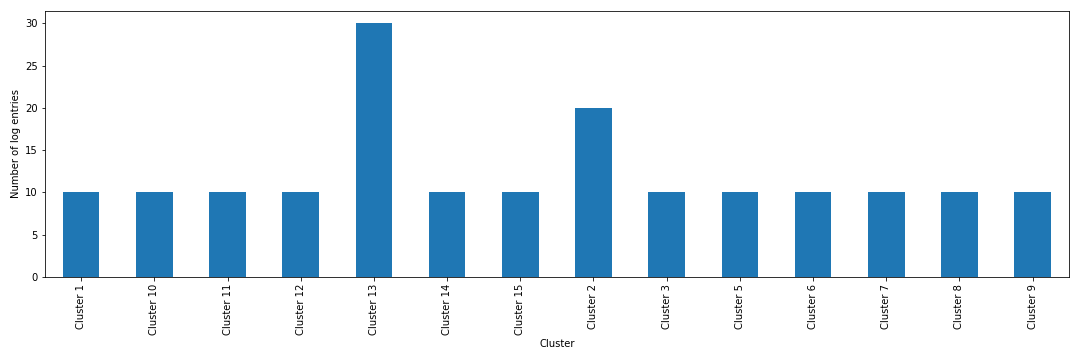
\includegraphics[scale=0.34]{labeled_eval}
	\caption{Clustered evaluation data set}\label{fig:eval-clustering}
\end{figure}

\subsection{Rand Index}
The \textit{Rand Index} in statistics, and in particular in data clustering, is a measure of the similarity between two data clusterings. Rand index is related to the accuracy, but is applicable even when class labels are not used. 
Mathematically Rand Index can be defined in the following way. 

Given a set \(S\) of \(n\) elements \(S = \{e_1,\dots,e_n\}\) and two partitions of \(S\) to compare. The first partition \(X = \{X_1,\dots,X_k\}\) into \(k\) clusters, and the second partition \(Y = \{Y_1,\dots,Y_l\}\) into \(l\) clusters. Define the following statements:
\begin{itemize}
	\item \(a\) -- the number of pairs of elements in the original set \(S\) that are in the \textbf{same} cluster in \(X\) and in the \textbf{same} cluster in \(Y\),
	\item \(b\) -- the number of pairs of elements in the original set \(S\) that are in \textbf{different} clusters in \(X\) and in the \textbf{same} cluster in \(Y\),
	\item \(c\) -- the number of pairs of elements in the original set \(S\) that are in the \textbf{same} cluster in \(X\) and in \textbf{different} clusters in \(Y\),
	\item \(d\) -- the number of pairs of elements in the original set \(S\) that are in \textbf{different} clusters in \(X\) and in \textbf{different} clusters in \(Y\).
\end{itemize}

Hence, the Rand Index, \(RI\) can be calculated as shown in Formula \ref{eq:rand-index} \cite{rand-index}:

\begin{equation}\label{eq:rand-index}
	RI = \frac{a + b}{a + b + c + d}
\end{equation}

The Rand index is often close to 1.0 even if the clusterings themselves differ significantly. In practice there often is a majority of element pairs that are assigned the different pair label under both the predicted and the ground truth clustering resulting in a high proportion of pair labels that agree, which leads subsequently to a high score\cite{quality-metrics}. Thus, the adjusted version of Random Index is commonly used in practice (Formula \ref{eq:adjusted-rand-index}). The adjusted Rand index is ensured to have a value close to 0.0 for random labeling independently of the number of clusters and samples and exactly 1.0 when the clusterings are identical (up to a permutation) \cite{adjusted-rand-index}.

\begin{equation}\label{eq:adjusted-rand-index}
	ARI = \frac{RI - E[RI]}{max(RI) - E[RI]},
\end{equation}
where \(E[RI]\) -- the expected \(RI\).

Easy to see that described above variables \(a\), \(b\), \(c\), \(d\) in their meaning correspond with \textit{True Positive (TP)}, \textit{False Positive (FP)}, \textit{False Negative (FN)}, \textit{True Negative (TN)} measures respectively, that are commonly used in \textit{Information Retrieval} area. And the Rand Index itself can be considered as \textit{accuracy} of clustering over the pairs of elements in \(S\).

These measures are used in classification tasks for comparing the results of the classifier that is being examined on some data set with ground truth labels that are known for this data set \cite{quality-metrics}. For clustering analysis, where ground truth labels, typically, are not known,  these metrics can be used as well since there is the evaluation data set, that was manually gathered and clustered from the server logs and could be considered as the ground truth.

Based on these measurements, a confusion matrix, presented on figure \ref{fig:confusion-matrix}, is built.

\begin{figure}[h!]\centering
	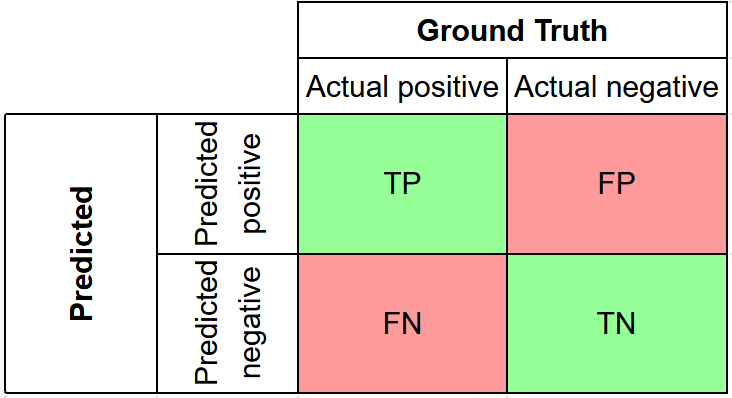
\includegraphics[scale=0.55]{confusion_matrix}
	\caption{Confusion matrix}\label{fig:confusion-matrix}
\end{figure}

Using \textit{TP}, \textit{FP}, \textit{FN}, \textit{TN} \textit{precision} (Formula \ref{eq:precision}) and \textit{recall} (Formula \ref{eq:recall}) metrics can be computed:
\begin{equation}\label{eq:precision}
	precision = \frac{TP}{TP + FP}
\end{equation}
\begin{equation}\label{eq:recall}
	recall = \frac{TP}{TP + FN}
\end{equation}

These metrics will be useful when comparing different log analytics methods.

\textit{Precision} can be interpreted as the ratio of pairs of log entries that were correctly grouped into the same cluster to the total number of pairs of log entries that were grouped into the same cluster by the algorithm.
While \textit{recall} is the ratio of pairs of log entries that were correctly grouped into the same cluster to the number of pairs log entries that were correctly grouped into the same cluster and the pairs log entries that were wrongly distributed among different clusters by the algorithm.

Thus in this thesis \textit{Adjusted Rand Index}, \textit{precision}, and \textit{recall} are chosen as clustering evaluation metrics.
\subsection{Linguistic approach}
In section \ref{sect:linguistic-approach} the linguistic approach to log analytics has been discussed. In this section the evaluation results of this approach are presented.

In the following table \ref{tab:evaluation-conditions-ling} the evaluation conditions including total number of log entries in the evaluation set, total target number of clusters that have been obtained from manual clustering of evaluation set, and total number of clusters that have been found by the considering algorithm.

\begin{table}[h!]\centering
	\caption{Linguistic approach evaluation}\label{tab:evaluation-conditions-ling}
	\begin{tabular}{ |c|c|c| }
		\hline
		\textbf{Total log entries} & \textbf{Target number of clusters} & \textbf{Total clusters found}\\
		\hline
		170 & 14 & 22 \\
		\hline
	\end{tabular}
\end{table}

%TODO
The linguistic method found 22 clusters, while the evaluation set consists of the log entries belonging to only 14 clusters. The log entries distribution among clusters obtained using the linguistic method is shown in Figure \ref{fig:eval-clustering-ling} This means that $\dots$ TBD

\begin{figure}[h!]\centering
	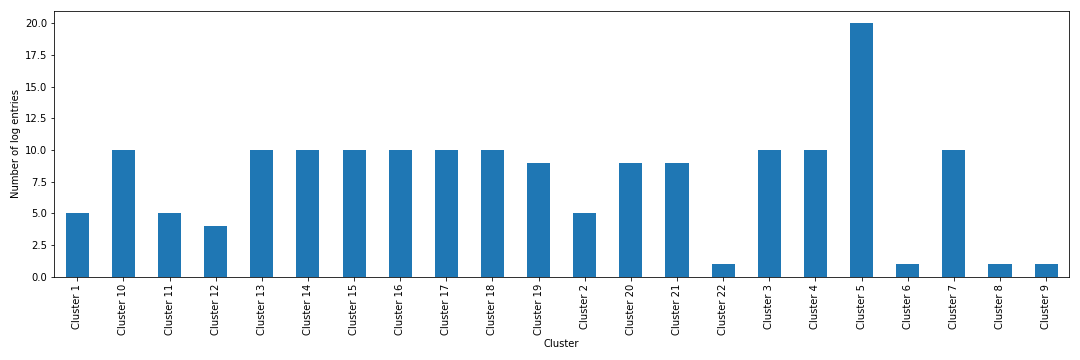
\includegraphics[scale=0.34]{nlp_eval}
	\caption{Linguistic approach clustering}\label{fig:eval-clustering-ling}
\end{figure}

% Total log entries to be evaluated: 170
% Total target number of clusters: 14
% Total clusters found: 22
% Precision: 0.9391796322489392
% Recall: 0.6041856232939036
% Accuracy: 0.9667246780368952
% F-measure: 0.7353266888150609
% RI: 0.9595544726766446
% ARI: 0.6810908320441991

% \pagebreak
In the Table \ref{tab:linguistic-evaluation} the evaluation metrics are presented.

\begin{table}[h!]\centering
	\caption{Linguistic approach evaluation}\label{tab:linguistic-evaluation}
	\begin{tabular}{ |m{9em}|m{4em}| }
		\hline
		\textbf{Metric} & \textbf{Result}\\
		\hline
		\textbf{Precision} & 0.94 \\
		\hline
		\textbf{Recall} & 0.61 \\
		\hline
		\textbf{ARI} & 0.69 \\
		\hline
	\end{tabular}
\end{table}

Relatively low recall score can be explained by the greater than it was expected number of found clusters. An increase in the number of clusters provoked an increase in the number of false negatives for log entries pairs which should be in the same cluster, but they were got into separate clusters.

Nevertheless, the precision score is high. That means the number of log entries pairs that were falsely grouped into the same cluster is low in comparison to the number of pair that were correctly grouped into the same cluster.

The overall accuracy of the algorithm is reflected in the ARI score that is equal to 0.69. 

\subsection{N-grams approach}
In this section the outcomes of the N-grams approach that has been described in section \ref{sect:n-grams-approach}  will be presented.

Similarly to the way it has been done in evaluation of the linguistic approach, the Table \ref{tab:evaluation-conditions-ngrams} is filled with the evaluation conditions including total number of log entries in the evaluation set, total target number of clusters that have been obtained from manual clustering of evaluation set, and total number of clusters that have been found by the N-grams algorithm.

\begin{table}[h!]\centering
	\caption{Linguistic approach evaluation}\label{tab:evaluation-conditions-ngrams}
	\begin{tabular}{ |c|c|c| }
		\hline
		\textbf{Total log entries} & \textbf{Target number of clusters} & \textbf{Total clusters found}\\
		\hline
		170 & 14 & 21 \\
		\hline
	\end{tabular}
\end{table}

In comparison with the linguistic approach the N-grams method grouped the evaluation data set into 21 clusters. This result, though not significantly, but closer to the target. The clustering with N-grams approach is depicted in Figure \ref{fig:eval-clustering-ngrams}.

\begin{figure}[h!]\centering
	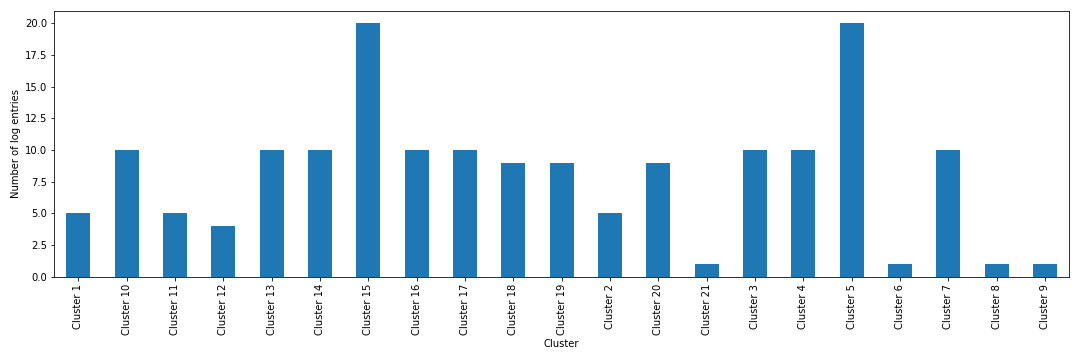
\includegraphics[scale=0.34]{ngrams_eval}
	\caption{N-grams approach clustering}\label{fig:eval-clustering-ngrams}
\end{figure}

Evaluation metrics are collected in the Table \ref{tab:evaluation-conditions-ngrams}.

\begin{table}[h!]\centering
	\caption{Linguistic approach evaluation}\label{tab:ngrams-evaluation}
	\begin{tabular}{ |m{9em}|m{4em}| }
		\hline
		\textbf{Metric} & \textbf{Result}\\
		\hline
		\textbf{Precision} & 0.95 \\
		\hline
		\textbf{Recall} & 0.70 \\
		\hline
		\textbf{ARI} & 0.75 \\
		\hline
	\end{tabular}
\end{table}

It can be seen that all characteristics have increased in comparison with the linguistic method. The precision of N-grams approach is 0.95 against 0.94 for the linguistic method, recall 0.70 against 0.61, and ARI 0.75 against 0.69. 

Such evaluation results tell that the N-grams method which does not rely on semantics, but works with log entries like with machine-generated text, shows better results and is a better choice when log clustering analysis is being performed.

\subsection{GSOM approach}
The third approach to log analytics is the GSOM. In this section the outcomes of this approach (the description of this approach is in %TODO
)
will be presented.


Total number of log entries in the evaluation set, total target number of clusters that have been obtained from manual clustering of evaluation set, and total number of clusters that have been found by the GSOM algorithm are presented in the Table \ref{tab:evaluation-conditions-gsom}.

\begin{table}[h!]\centering
	\caption{Linguistic approach evaluation}\label{tab:evaluation-conditions-gsom}
	\begin{tabular}{ |c|c|c| }
		\hline
		\textbf{Total log entries} & \textbf{Target number of clusters} & \textbf{Total clusters found}\\
		\hline
		170 & 14 & 14 \\
		\hline
	\end{tabular}
\end{table}

Unlike linguistic and N-grams methods GSOM has found 14 clusters that corresponds with the target number. The diagram of log entries distribution among clusters is shown in Figure \ref{fig:eval-clustering-gsom}.

\begin{figure}[h!]\centering
	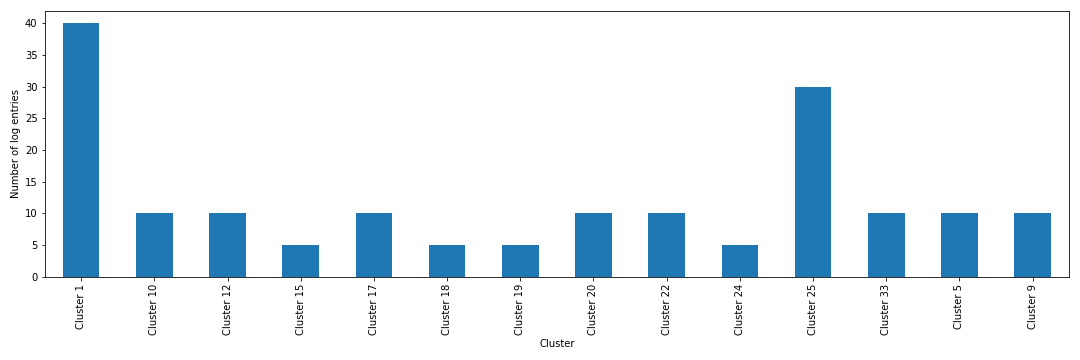
\includegraphics[scale=0.34]{gsom_eval}
	\caption{GSOM approach clustering}\label{fig:eval-clustering-gsom}
\end{figure}

When observing clustering bar diagram (Figure \ref{fig:eval-clustering-gsom}) it can be seen that "Cluster 1" contains 40 log entries. No one cluster in manually clustered evaluation data set (Figure \ref{fig:eval-clustering}) does not contain such a number of log entries. 10 log entries that belong to another cluster in evaluation data set have been assigned to "Cluster 1" by the GSOM.

Evaluation metrics are collected in the Table \ref{tab:evaluation-conditions-gsom}.

\begin{table}[h!]\centering
	\caption{GSOM approach evaluation}\label{tab:gsom-evaluation}
	\begin{tabular}{ |m{9em}|m{4em}| }
		\hline
		\textbf{Metric} & \textbf{Result}\\
		\hline
		\textbf{Precision} & 0.75 \\
		\hline
		\textbf{Recall} & 0.97 \\
		\hline
		\textbf{ARI} & 0.78 \\
		\hline
	\end{tabular}
\end{table}

In comparison with both previous method, GSOM shows significantly better results in recall, 0.97 against 0.70 and 0.61 for N-grams and linguistic methods respectively. Precision score, on the contrary, have been decreased against N-grams and linguistic approaches, where the recall score was 0.95 and 0.94 respectively. Nevertheless, the ARI score of GSOM method is higher than 0.75 and 0.69 for N-grams and linguistic methods.

GSOM affects the FN score in the sense that the number of log entries pairs that should not be grouped into the same cluster are not actually grouped. But some log entries were misclusterd into the same cluster, and hence the FP score increased. And because of this the precision score decreased.


\subsection{Evaluation summary}
In this section the results of evaluation of three different approaches to log analytics were discussed.

According to these results N-grams method is a better choice for log analytics purposes since is has better precision score in comparison with linguistic approach and GSOM. Time elapsed for N-grams clustering is better than the corresponding value in linguistic method since the N-grams vectorization process is simpler then linguistic vectorization, it is free of time consuming normalization phases such as, for instance, stemming. %TODO check whether stemming can be time consumable...

GSOM is another good method and potentially it could be the best one, but it has some limitations that makes the usability of this approach more difficult. For example, for better clustering with this method, it must be trained on large enough and qualitative training data set that should cover as many probable log entries as possible. Another limitation is the training process itself. Typically for machine learning methods in general and neural networks in particular the training process requires a large number of iterations that in couple with large training data set forms a complex task.

\setsecnumdepth{part}
\chapter{Conclusion}


\bibliographystyle{iso690}
\bibliography{mybibliographyfile2}

\setsecnumdepth{all}
\appendix

\chapter{Acronyms}
% \printglossaries
\begin{description}
	\item[NLP] Natural Language Processing
	\item[XML] Extensible markup language
\end{description}


\chapter{Contents of enclosed CD}

%change appropriately

\begin{figure}
	\dirtree{%
		.1 readme.txt\DTcomment{the file with CD contents description}.
		.1 exe\DTcomment{the directory with executables}.
		.1 src\DTcomment{the directory of source codes}.
		.2 wbdcm\DTcomment{implementation sources}.
		.2 thesis\DTcomment{the directory of \LaTeX{} source codes of the thesis}.
		.1 text\DTcomment{the thesis text directory}.
		.2 thesis.pdf\DTcomment{the thesis text in PDF format}.
		.2 thesis.ps\DTcomment{the thesis text in PS format}.
	}
\end{figure}

\end{document}
